\section{Experiment}\label{sec:method}
\subsection{Method}
In order to test if our product helps solve our product statement, we wish
to make an experiment that quantitatively evaluates the effectiveness of our
program. 

In order to do this, we have devised the following experiment:
\begin{figure}[H]
  \centering
  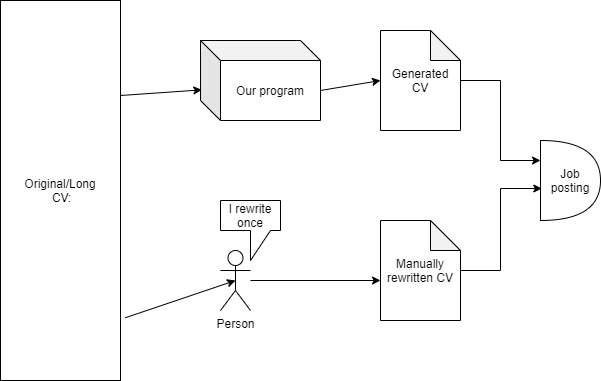
\includegraphics[scale = 0.6]{figures/experiment1.png}
  \caption{Experiment Method}\label{fig:ie}
\end{figure} 
In the experiment we will create a long CV where all the original information
is in. We do this to ensure that there is no extra information in the human 
rewritten CV that our program couldn't have created. In this way, we ensure
the test is as fair as possible.

Thereafter the danish job center will be asked, to answer which of the two CV's is most suited
for the job posting. How this works is as such:
\\
The human will shorten down and create a CV based on the long CV. This CV is
is gonna be compared to n number of job postings.
Our program, is gonna filter down the long CV, and create a job application,
for each individual job posting. 
To ensure, that some job postings don't just have lower requirements, we will be
comparing the new CV applications from both the program and the person to the same 
job postings each time. In total we will be comparing n number of applications.
\\
In this way, we can assume that both the human who had rewritten one
CV and the program, who has rewritten n number of CV's,
will take about the same amount of time, to create n CV's .
Therefore we can somewhat ensure that the results are somewhat fair, in relation to the amount of effort each set of n CV's require.
The structure of both CV's should also remain the same in the testing, such that one CV isn't prioritized because of better formatting.
This is important, since the test is primarily testing the CV's contents compared to the job opening.
\\
This experiment will compare the results of how many times one gets a "job
interview" using one of the two methods: Comparing the amount of 
"job interviews" (based on what the job center thinks is most likely to earn an interview) 
from the qualitatively created CV from
the human, to the quantitatively created CV from the program to
each other.
\\
The results from this, will be a good indication, whether our program solved, or
at least helped, in the process of getting a job interview, or if just manually
creating one good application is better.

\subsection{Results}
After we were finished with the program, we decided to print out one CV that has been made by a human,
and six almost identical CV to each other the only differences is 
the background information is matching to each keyword there is in the any job posting there is, 
therefore some of the text has different priorities for the CV. \\

We went to the job center to ask a job counselor about whether a human CV can match up against a computer.
The female job counselor agreed to check our CVs, and afterwords give these feedbacks. 
She saw the human CV first, and it was graded to have fine structure,
also there are a fine red thread to fine the flow of the CV, 
but there were some deep thoughts about inserting "I" at the start of almost every sentences, 
so we didn't balance the part with limited amount of "I"s.
The ATS scanner will not necessarily decline the CV, also there can be scenarios where people would like to have variations of CVs.
This way it is going to be too descriptive for a recruiter to read. 
In comes as no surprise that this human made CV should have some qualities for more structure than contents.
As a matter of fact more and more of the text can be ignored, if a person is going to apply for a high ranking position. \\

It's was fine to have bullet points for the education and work experience parts, so that was a success, 
and that goes for both the human and computer CV.
It gave the job counselor a good impression of how it was structured instead of doing the same as the free text.
If text didn't have any spaces at all the recruiter will most likely throw it out before even reading it, 
because of how it could be structured. It is important to note that education and work experience is most likely to be required for a passing grade. 
On the other hand some jobs doesn't required any working experience and professional skills from a education, 
and these job could be like a supermarket position. \\

An important note is that when the job counselor look at the CVs closer, 
she thought about one of the CV was clearly made by a computer without any guidance from the group,
and after she saw three of the computer made CVs, she instantly pointed out even though the human and computer made CV have the same characteristics
they still have a clear difference for structure and contents. 
She pointed out the human made has flaws about the contents, since it was again too descriptive, 
therefore this CV could gain a higher chance of getting a recruiter to like it
if there was less contents and more structure, and the computer could have more contents instead of structure.

% Spørg om hvis menneske cv'et manglede 
%Husk at spørge om hvad rød tråd er på engelsk.